\documentclass{standalone}
  \usepackage{tikz}
  \usetikzlibrary{arrows.meta, automata, bending, positioning, shapes.misc}
  \tikzstyle{automaton}=[shorten >=1pt, >={Stealth[bend,round]}, initial text=]
  \tikzstyle{accepting}=[accepting by arrow]

\begin{document}
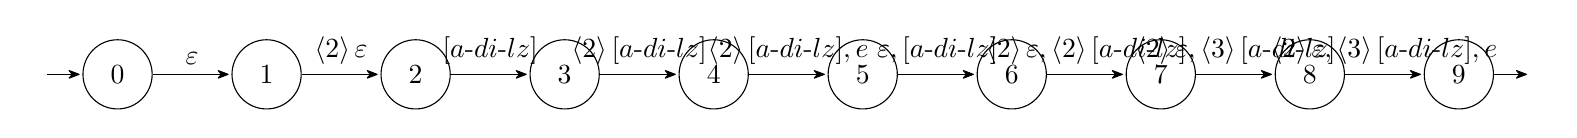
\begin{tikzpicture}[automaton, auto]
  \node[state,initial] (0) {$0$};
  \node[state] (1) [right=of 0] {$1$};
  \node[state] (2) [right=of 1] {$2$};
  \node[state] (3) [right=of 2] {$3$};
  \node[state] (4) [right=of 3] {$4$};
  \node[state] (5) [right=of 4] {$5$};
  \node[state] (6) [right=of 5] {$6$};
  \node[state] (7) [right=of 6] {$7$};
  \node[state] (8) [right=of 7] {$8$};
  \node[state,accepting] (9) [right=of 8] {$9$};
  \path[->] (0) edge node {$\varepsilon$} (1);
  \path[->] (1) edge node {$\left\langle 2\right\rangle \varepsilon$} (2);
  \path[->] (2) edge node {$[a\textrm{-}di\textrm{-}lz]$} (3);
  \path[->] (3) edge node {$\left\langle 2\right\rangle [a\textrm{-}di\textrm{-}lz]$} (4);
  \path[->] (4) edge node {$\left\langle 2\right\rangle [a\textrm{-}di\textrm{-}lz], e$} (5);
  \path[->] (5) edge node {$\varepsilon, [a\textrm{-}di\textrm{-}lz]$} (6);
  \path[->] (6) edge node {$\left\langle 2\right\rangle \varepsilon, \left\langle 2\right\rangle [a\textrm{-}di\textrm{-}lz]$} (7);
  \path[->] (7) edge node {$\left\langle 2\right\rangle \varepsilon, \left\langle 3\right\rangle [a\textrm{-}di\textrm{-}lz]$} (8);
  \path[->] (8) edge node {$\left\langle 2\right\rangle \varepsilon, \left\langle 3\right\rangle [a\textrm{-}di\textrm{-}lz], e$} (9);
\end{tikzpicture}
\end{document}
